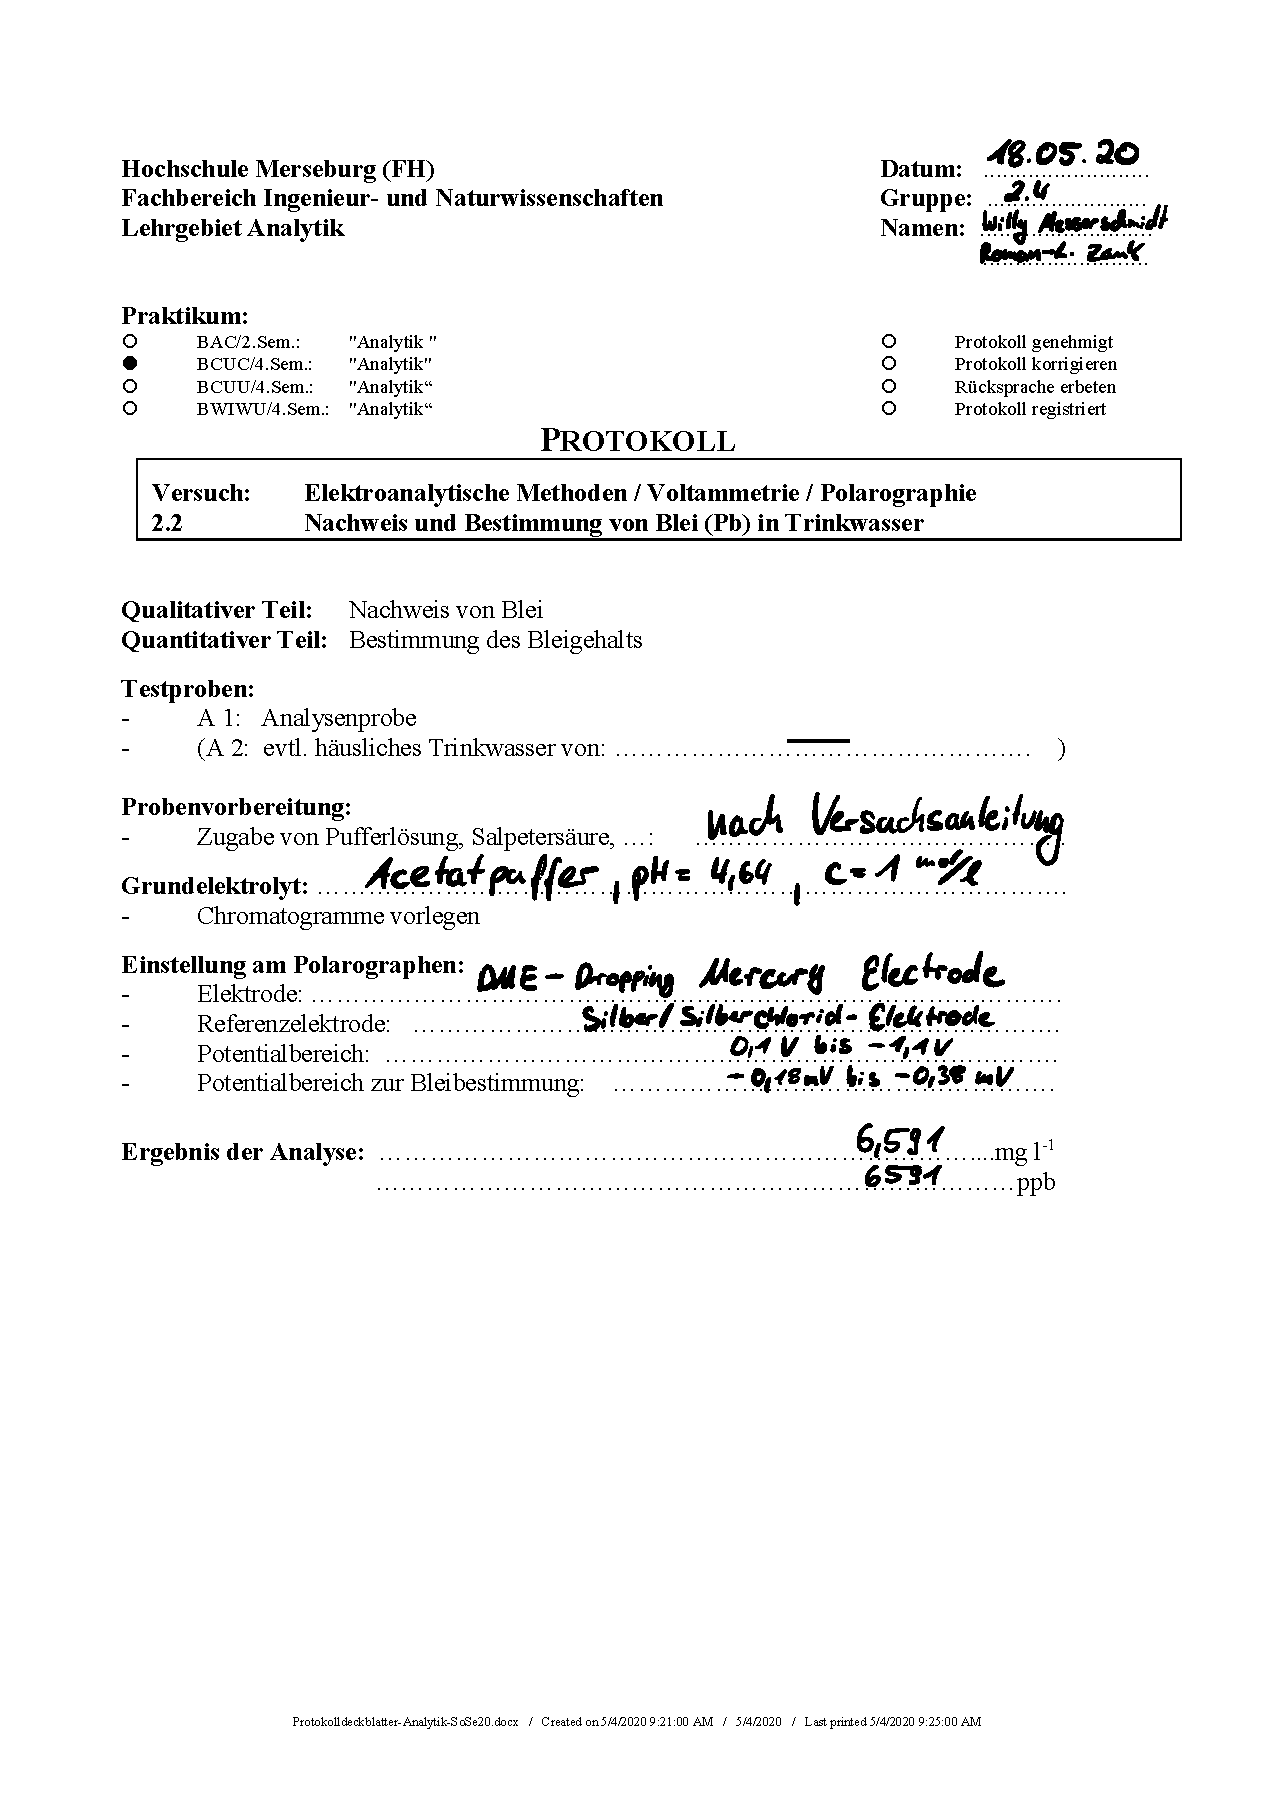
\includepdf[]{Deckblatt}
\section{Einleitung}
\label{sec:einleitung}
%Beschreibung der Grundzüge der Polarographie

Als Teil der Voltammetrie bezeichnet die Polarographie ein Analyseverfahren, bei dem eine tropfende Quecksilberelektrode als polarisierbare Elektrode genutzt wird (siehe Abb. \ref{fig:schema_polarograph}). Die im Praktikum aufgenommenen Daten beinhalten die \mbox{Stromstärke $I$} als Messgröße über die angelegte \mbox{Gleichspannung $U$} als variierende Größe. Das Verfahren beruht dabei auf der elektrolytischen Abscheidung, in diesem Fall Reduktion, von Stoffen aus der Probenlösung.\cite{Brehm.2004}

%Start
\begin{figure}[h!]
	\centering
	\includegraphics[width=0.4\textwidth]{img/Polarograph}
	\caption{Schematische Darstellung eines Polarographen \cite{Brehm.2004}}
	\label{fig:schema_polarograph}
\end{figure}
\FloatBarrier
%Ende

Im Versuch wurde mittels des Analyseverfahrens der Polarographie, der Bleigehalt in einer unbekannten Wasserprobe bestimmt.